\subsection{TPMD is labour intensive}

\paragraph{Designing microbenchmarks} 
We start the process of TPMD by first identifying the list of {\it power model parameters}
for CPU and GPU, as listed in Table~\ref{tab:parameters}.
% \paragraph{Parameters of the CPU and GPU power models.}
% Pixel2, Moto Z3~\cite{motoz3} and Pixel 4 are representative of modern smartphones
% that uses the big.LITTLE CPU architecture~\cite{biglittlearch} to
% provide energy efficiency in supporting diverse workloads.
% Particularly, in Pixel 2 and Moto Z3, the LITTLE cores can operate in 22 different frequencies 
% and big cores can operate in 31 different frequencies.
% Whereas, for Pixel 4, the LITTLE cores can operate in 18 different frequencies 
% and big cores can operate in 20 different frequencies.
%  The cores are switched to higher frequencies when higher performance is required.
% At runtime, the OS scheduler along with the CPU governor performs power state transition and core frequency scaling to optimize the CPU energy draw as the workload varies.
From~\cite{multicoremodel:2015}, the parameters of the CPU power model include
the base power consumed $p_{\text{base}}$ when the cores are idle and
the non-base core $i$ power running at frequency $f_k$, $p^c_i(f_k)$.
%, as listed in Table~\ref{tab:parameters}.
% The total CPU power can be modeled as:
% {
% \begin{equation}
%     P_{\text{CPU}} = p^c_{\text{base}} + \sum_{i} p^c_i(f_k)
% \end{equation}
% 
% }
% In Moto Z3, 
% GPU can run at different frequencies and can either be busy or idle.
% has three power states, Active, Slumber, and Aware.
% Since the GPU never enters the Slumber or Aware state when an app is running, 
The parameters of the GPU model include the GPU power draw in 
% Active-busy and Active-idle 
busy and idle states in each frequency, $p^g_{\text{busy}}(g_k)$ and 
$p^g_{\text{idle}}(g_k)$.
% We abbreviate Active-busy and Active-idle states simply
% as GPU Busy and Idle states in the rest of the paper.

% \if 0
% Accordingly, we model the GPU power draw as follows:
% \begin{equation}
%     Power_{GPU} = \sum_{j}\sum_{i} u_{ij}*p_{ij}
%     \end{equation}
% where $p_{ij}$ is the power parameter for the $i^{th}$ GPU frequency for the $j^{th}$ power state (Active-busy, Active-idle, Slumber, Aware) and $u_{ij}$ is the corresponding utilization in that frequency and power state.
% \fi

%\paragraph{TPMD methodology.}
We design CPU microbenchmarks that perform 
arithmetic and memory operations for 7 seconds each 
with 100\% utilization.

\begin{sloppy}
For the GPU, we first used a third-party rendering benchmark 3DMark~\cite{3DMark}. 
	But on running the benchmark, we found that 3DMark renders quite different
	consecutive frames which result in rapidly fluctuating GPU utilizations and
	power monitor readings, making the alignment \comment{of what?? of
	the 16.7 ms GPU rendering intervals wrt the power monitor as each rame has a different GPU utilization} difficult. 
\end{sloppy}
In contrast, we observed that real apps tend to render very similar consecutive
frames in a short period of time which result in relatively stable GPU
utilization and stable total power draw, making it easier to extract the power
monitor reading corresponding to a given GPU utilization (see
Figure~\ref{fig:power_trace_candycrush_menu} later).  Thus, we directly used
selected apps that use only the CPU and GPU to derive the GPU power models.  In
particular, we derive the CPU model by first using the 
% integer-arithmetic 
CPU arithmetic microbenchmark\footnote{We found using the CPU model derived
using memory-intensive microbenchmark resulted in negative GPU coefficients.}
and then using the difference between the measured phone power and
model-estimated CPU power when running an app as the ground-truth for the GPU
power draw and GPU power model derivation.


\paragraph{Running microbenchmarks}
\aj{We first prepared the three phones by connecting power monitor and bypassing 
the battery interface.} \comment{Were there some challenges here for separate 
device models?}
\dcomment {
We faced different challenges while attaching each device to the power monitor
\eg attaching the power monitor leads to power management circuit .
}

We ran the CPU microbenchmark while fixing the big core cluster at each 
of the 31 frequencies
for both Pixel 2 and Moto Z3 and at each of the 20 frequencies for Pixel 4, 
on 1 core and 2 cores.
% When using 1 core, 2 cores and 4 cores, the remaining cores are offline.
We measure the base CPU power as the phone power draw when all cores are idle.
We manually align the power monitor readings for each of the 7-second interval 
and derive the non-base per-core power for each frequency by 
subtracting the base power from the measured total phone power.
\comment{This is not bad? Only (7+7)*31 = ~7 minutes of run. Do we have to repeat
it multiple times or something else that makes it LABORIOUS?
}
\dcomment{
For the purpose for this paper we considered only 2 big cores for the ease of our experiments.
While in the real world scenario the device has to profiled on all states \ie
taking into account the interaction between the LITTLE core and big cores.
There are in total 24 configuration of cores for Pixel 2 in which they can be
online ( for a 4 LITTLE cores 0 to 4 cores could be active, same for big cores,
remove the case where both cores are offline).
As there are 22 LITTLE core and 31 big core frequencies we further have $22x31=682$
combination. Using our methodology it could take up to $24x682x7$ seconds = 1.33 days for
just to gather the required measurements.
}
% After running
% the benchmarks, we found that for all the
% phones, 
% %we found that 
% the per-core power $p_i(f_k)$ remains the same for different cores.

% Similar to CPU, the GPU of modern smartphones have also vastly developed.
% Initially, we tried to use a GPU benchmark, 3DMark~\cite{3DMark}, to drive the GPU usage into Busy and Idle states under each frequency.
%
% This makes aligning the power monitor readings with the GPU Busy periods difficult
% which is needed to extract the GPU Busy state power at each frequency.
%
%  the rendering task often finishes in less than the 16.7ms per-frame interval and hence the GPU will go through busy and idle states in every 16.7ms interval, making it much easier to manually identity both states. 
% \questionaj{Why do we have to identify manually? Triggers are not available in atrace?
% Due to both drift and scaling their is vast alignment problem in aligning each 16.7 ms interval.
% Alignment problem prevent us from directly using triggers from the event trace.}

% 5. Explain results and observation

\begin{figure*}[tp]
    \centering
     \begin{subfigure}[b]{0.32\textwidth}
         \centering
         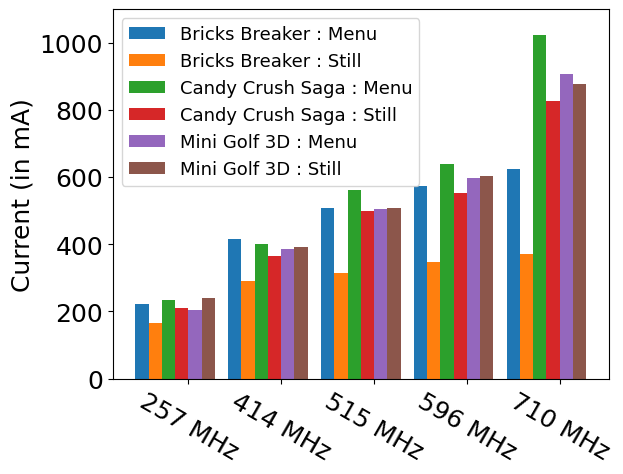
\includegraphics[width=\textwidth]{figures/002_Pixel2_gpu_model.png}
         \caption{Pixel 2}
         \label{fig:gpu_model_p2}
     \end{subfigure}
    \begin{subfigure}[b]{0.32\textwidth}
         \centering
         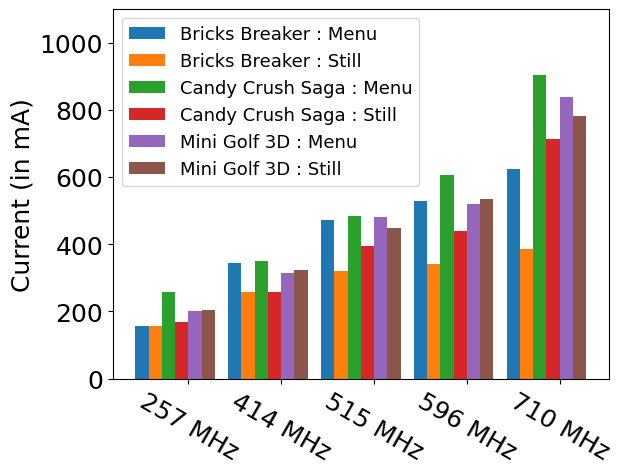
\includegraphics[width=\textwidth]{figures/003_MotoZ3_gpu_model.png}
         \caption{Moto Z3}
         \label{fig:gpu_model_z3}
     \end{subfigure}
    \begin{subfigure}[b]{0.32\textwidth}
         \centering
         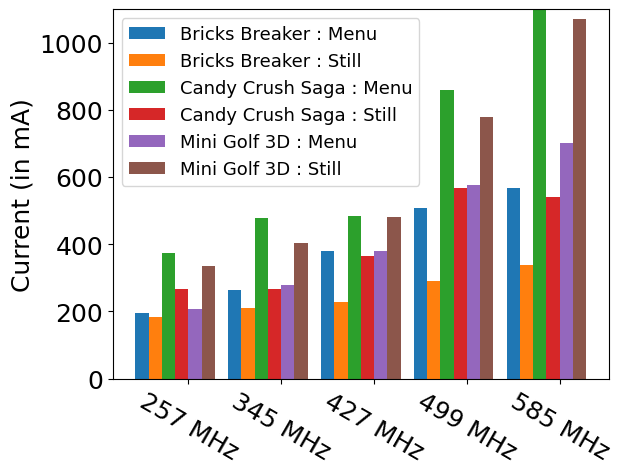
\includegraphics[width=\textwidth]{figures/004_Pixel4_gpu_model.png}
         \caption{Pixel 4}
         \label{fig:gpu_model_p4}
     \end{subfigure}
     \hfill
    \caption{TPMD-derived GPU power model (only Busy power is shown) with
        the CPU frequency fixed at 1.42 GHz for both Pixel 2 and Moto Z3,
        and 1.61 GHz for Pixel 4. ??? FIXED}
    \label{fig:gpu_model}
    \vspace{-0.1in}
\end{figure*}

\begin{table*}[tb]
    \caption{Energy estimation error (\%) for app scenarios 
    using the GPU model derived for each scenario with CPU and GPU frequencies fixed for the 3 phones. (B: Bricks Breaker, C: Candy Crush Saga and M: Mini Golf 3D)}
    \vspace{-0.1in}
    \centering
    \begin{subfigure}[b]{0.31\textwidth}
        \caption{Pixel 2}
        \vspace{-0.05in}
        \centering
    	{ \scriptsize
    	\begin{tabular}{ | p{10.8mm} | c | c | c | c | c | c | }
    		\hline
    		     & \multicolumn{6}{ c|}{Error for each App Sc. (\%)}\\ % \multicolumn{6}{ c|}{Error for each App Scenarios (\%)}\\
    		\cline{2-7}
                    Model & \rot{B. Menu} & \rot{B. Still} & \rot{C. Menu} & \rot{C. Still} & \rot{M. Menu} & \rot{M. Still}  \\
    		\hline
                B. Menu              & 8.9 & 13 & 20 & 16 & 11 & 14 \\
                B. Still             & 15 & 11 & 31 & 25 & 17 & 26 \\
                C. Menu              & 16 & 24 & 11 & 11 & 13 & 11 \\
                C. Still             & 16 & 19 & 14 & 12 & 12 & 14 \\
                M. Menu              & 9.9 & 14 & 14 & 11 & 8.1 & 11 \\
                M. Still             & 12 & 21 & 9.7 & 10 & 11 & 8.6 \\
    		\hline
    	\end{tabular}
    	}
    \end{subfigure}
    \hfill
    \begin{subfigure}[b]{0.31\textwidth}
        \caption{Moto Z3}
        \vspace{-0.05in}
        \centering
    	{ \scriptsize
    	\begin{tabular}{ | p{10.8mm} | c | c | c | c | c | c | }
    		\hline
    		     & \multicolumn{6}{ c|}{Error for each App Sc. (\%)}\\ % \multicolumn{6}{ c|}{Error for each App Scenarios (\%)}\\
    		\cline{2-7}
                    Model & \rot{B. Menu} & \rot{B. Still} & \rot{C. Menu} & \rot{C. Still} & \rot{M. Menu} & \rot{M. Still}  \\
    		\hline
                B. Menu              & 16 & 18 & 44 & 18 & 22 & 25 \\
                B. Still             & 18 & 15 & 36 & 15 & 17 & 17 \\
                C. Menu              & 30 & 24 & 16 & 23 & 18 & 16 \\
                C. Still             & 12 & 12 & 31 & 11 & 15 & 17 \\
                M. Menu              & 18 & 16 & 23 & 15 & 14 & 15 \\
                M. Still             & 20 & 15 & 20 & 14 & 12 & 13 \\
    		\hline
    	\end{tabular}
    	}
    \end{subfigure}
    \hfill
    \begin{subfigure}[b]{0.31\textwidth}
        \caption{Pixel 4}
        \vspace{-0.05in}
        \centering
    	{ \scriptsize
    	\begin{tabular}{ | p{10.8mm} | c | c | c | c | c | c | }
    		\hline
    		     & \multicolumn{6}{ c|}{Error for each App Sc. (\%)}\\ % \multicolumn{6}{ c|}{Error for each App Scenarios (\%)}\\
    		\cline{2-7}
                    Model & \rot{B. Menu} & \rot{B. Still} & \rot{C. Menu} & \rot{C. Still} & \rot{M. Menu} & \rot{M. Still}  \\
    		\hline
                B. Menu              & 15 & 15 & 44 & 19 & 15 & 34 \\
                B. Still             & 15 & 15 & 50 & 23 & 17 & 40 \\
                C. Menu              & 30 & 33 & 12 & 20 & 25 & 13 \\
                C. Still             & 18 & 20 & 25 & 15 & 16 & 19 \\
                M. Menu              & 15 & 16 & 34 & 17 & 14 & 26 \\
                M. Still             & 25 & 28 & 13 & 15 & 21 & 12 \\
    		\hline
    	\end{tabular}
    	}
    \end{subfigure}
    \label{tab:gpu_model_error}
    \vspace{-0.1in}
\end{table*}
% Comparison Table for GPU model with other scenarios Here

For GPU model derivation, we repeated runs for three popular games apps,
Bricks Breaker, Candy Crush Saga and Mini Golf 3D, each running two
scenarios, as listed in Table~\ref{tab:app_scenario_description}.  To
minimize the variance of CPU power draw, we fixed the CPU frequency at
1.42 GHz for both Pixel 2 and Moto Z3, and 1.61 GHz for Pixel 4, and ran
each of the app scenario under each GPU frequency for a duration of 30
seconds.
\comment{Again, not not bad. What makes this process LABORIOUS?}
\dcomment {
The GPU model derivation has to be derived for each app the user requires.
Making this impossible to device manufactures to model GPU in it entirely
as there are billions of apps presents currently.
}

\subsection{TPMD is not comprehensive}

Our CPU modeling results (details omitted) show that
the CPU power draw for the arithmetic-intensive and memory-intensive
operations of the microbenchmark differ significantly,
by 38.7\% at 300 MHz and 56.8\% at 2.45 GHz for Moto Z3.
This suggests that the arithmetic-memory operation mix can send the CPU cores
to different power state variations, draining different amount of power.

Figure~\ref{fig:gpu_model}(a)-(c) shows the derived power models 
for varying GPU frequencies for the 3 phones. 
Only GPU Busy power are shown due to page limit.
% The full bars represent the busy current whereas the solid bars are the idle current.
% and Table~\ref{tab:gpumodel_nexus6} for Nexus 6.
%% 5a. Explain per scenario dependent modeling
We make two observations.
%
(1) The GPU power parameters for the same frequency differ with {\it
different apps}. For example, on Moto Z3 at 710 MHz, the GPU Busy power draw for
Bricks Breaker Still is 57.2\% lower than for Candy Crush Saga Menu.
%
(2) The GPU power parameters for the same frequency even differ for
{\it different scenarios} of the same app. For example, for Bricks Breaker, the GPU
Busy power draw for the Still scenario is 32.3\% and 35.5\% lower than
for the Menu scenario at 515 MHz and 596 MHz, respectively, on Moto Z3.
Similar observations can be made about the other two phones.

%% 5b. Explain the reasons for the observation
The above dependence of the GPU power draw on app usage can be
attributed to two main reasons.  (1) The GPU has a large number of
mini-cores, but the utilization metric available to the OS only
captures the temporal utilization and not the spatial utilization, \ie
the percentage of mini-cores those were active.  Different spatial
utilization may drive the GPU into different power state variations
that have the same temporal utilization but different power draw.
% 
(2) Using a single CPU model in estimating the CPU power draw which is
 to be subtracted from the total phone power may result in errors in
 the GPU power draw estimation, as rendering different frames for
 different app scenarios (of the same or different apps) may result in
 different CPU usage, \eg due to different mix of arithmetic and
 memory operations and hence CPU power draw.  Such error propagation
 happens in TPMD which models one component at a time and often relies
 on the models of a prior component to estimate the "ground truth" in
 modeling the next component.

% \paragraph{Cross validation.}
To further demonstrate that the GPU models derived per app scenario captures
the model dependence on the app usage also, we perform a cross validation
by applying the GPU model derived from each of the six app scenarios
shown in Figure~\ref{fig:gpu_model}(a)-(c) to estimate the total
energy of all app scenarios (including self).
Tables~\ref{tab:gpu_model_error}(a)-(c) shows the results for 
the case where the CPU frequency is fixed at 1.42 GHz for Pixel 2 and Moto Z3 and 1.61 GHz for Pixel 4, and the GPU frequency is fixed at 257 MHz for all three phones.
We observe that the energy estimation error
is much lower when the GPU model derived for an app scenario is
applied to itself (diagonal values), ranging between 
8.09\%-11.56\% for Pixel 2,
11.47\%-16.25\% for Moto Z3, and
11.90\%-15.21\% for Pixel 4,
than when a model derived for one scenario is applied
to other scenarios (off-diagonal values), which
range between 
9.73\%-31.26\%,
11.57\%-44.25\%, and
13.07\%-50.43\%.


% \comment{
% We observe that the lowest error for a scenario is
% due to GPU model derived from same scenario (fitting error), whereas for
% all other scenario GPU models the error can be as much as 2$times$ higher.
% For the higher GPU frequencies, like 710 MHz the difference in the can increase up to about 10 times.
% }


\if 0
we calculated the error
in estimating the total GPU energy drain in the second scenario of each app 
if using the GPU model derived using the first scenario of each app.
The rows labelled "GPU energy error" in Table~\ref{tab:gpumodel_motoz3} shows that the error ranges between ??\%--??\%, ??\%--??\%, and ??\%--??\% for the second scenarios of the three apps.
\fi





